\subsubsection{USB-B}
\label{subsubsec:Inbetriebnahme_USB-B}

Für die Inbetriebnahme der USB-B-Schnittstelle wurde vorerst geprüft, ob der USB-UART-Converter über die USB-Buchse und Kabel vom Computer erkannt wird. Danach wurde geprüft, wie der Handshake beim Programmieren der Komponenten funktioniert. Die Inbetriebnahme der Programmierung wird in den Kapitel \ref{subsubsec:Inbetriebnahme_ESP} (WiFi-Modul) und Kapitel \ref{subsubsec:Inbetriebnahme_uC_Vorgehen} (Mikrocontroller) beschrieben. Dies geschieht ein wenig parallel, denn die Programme zum Schreiben, Kompilieren und Hochladen des Codes müssen schon vor dem Prüfen der USB-B-Schnittstelle installiert sein. Für die Inbetriebnahme wurde entschieden, dass der Handshake noch zum USB-B-Teil gehört und als Voraussetzung zählt, sodass das Programm überhaupt hochgeladen werden kann. Ausserdem wird dieser Handshake unabhängig davon gemacht, ob ein Device angehäng ist oder nicht. Erst nach einer Überprüfung der Device-Nummer kann bestimmt werden, ob das Target (ESP32 und ATMega2560) vorhanden ist oder nicht. Um den Handshake zu kontrollieren sind die in Abbildung \ref{fig:USB_B_Print} eingekreisten Punkte interessant:


\begin{figure}[h!]
\center
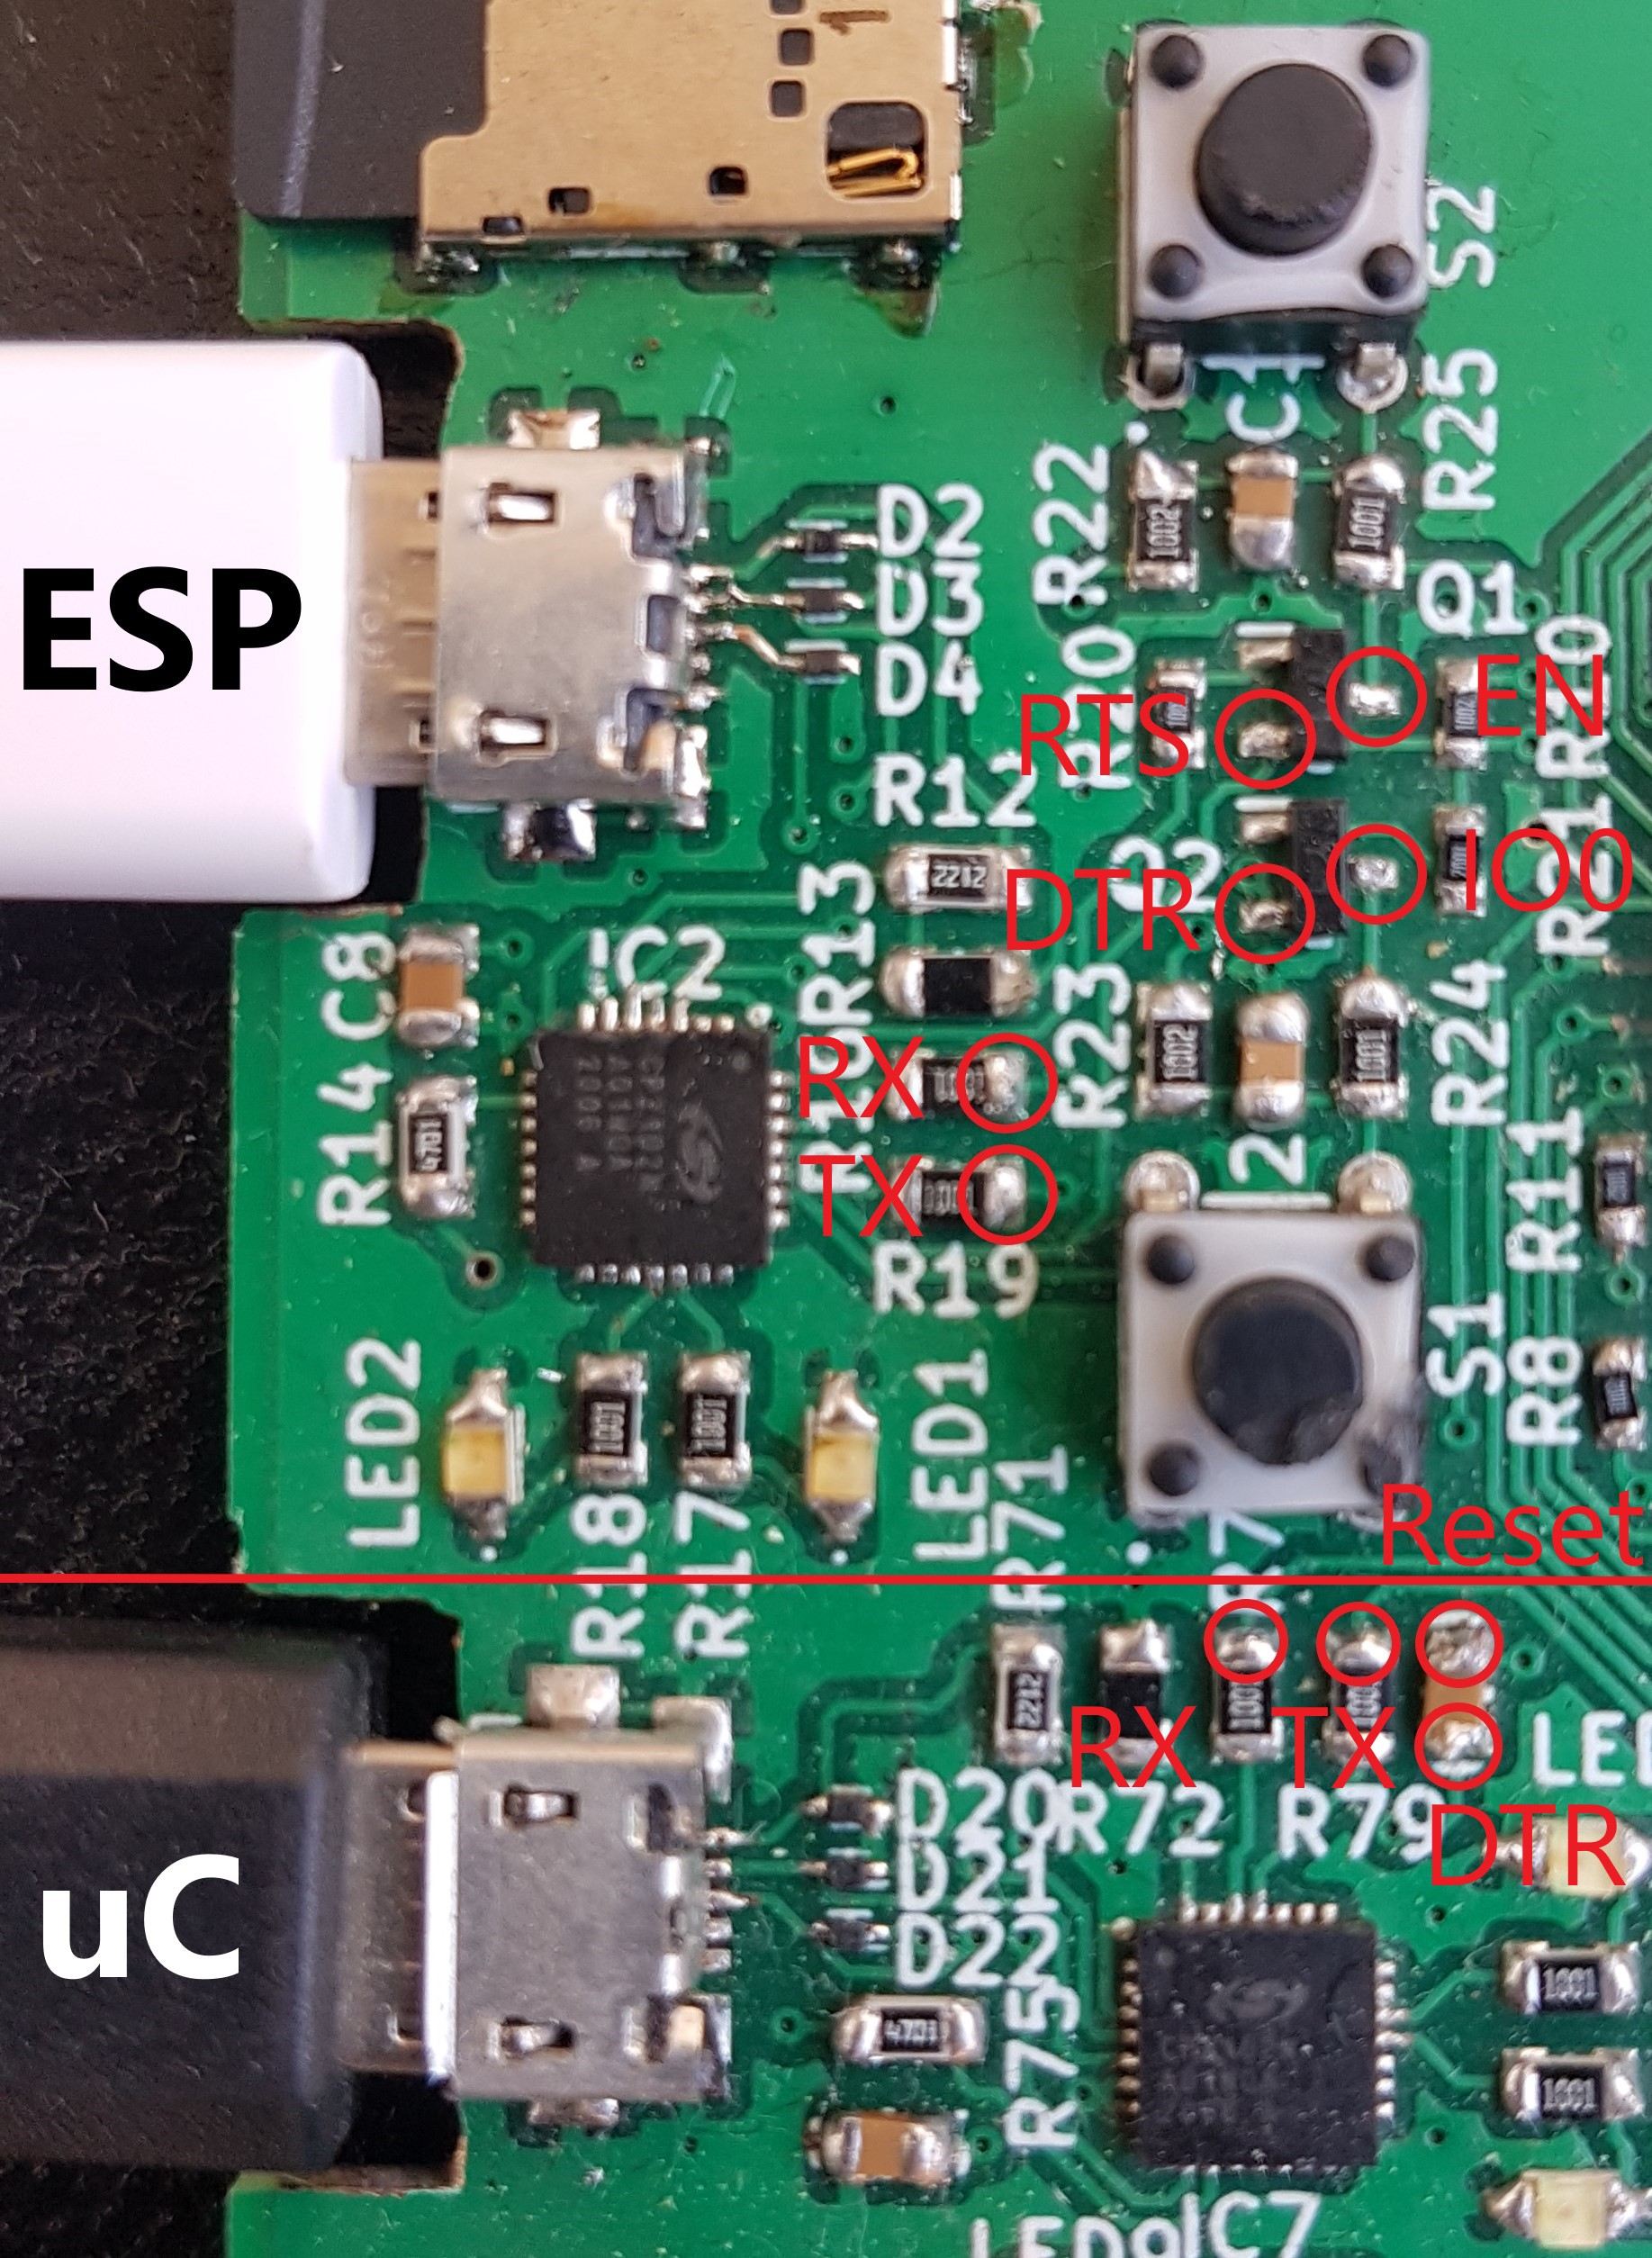
\includegraphics[width = 0.58\textwidth]{graphics/USB_B_Print}
\caption{Ausschnitt aus Platine (USB-Scnittstellen) mit eingekreisten Messpunkten.}
\label{fig:USB_B_Print}
\end{figure}
\newpage
Folgende Schritte wurden befolgt:

\begin{enumerate}
\item Platine mit Spannung versorgen und Computer mit zwei USB-Kabeln an die USB-B-Buchsen anschliessen.\\
\textcolor{blue}{Systemeinstellungen \textrightarrow Geräte-Manager} (siehe Abbildung \ref{fig:USB_Devices_Ger_Man})\\
Dort sind die Devices sichtbar unter dem Name: \textit{Silicon Labs CP210x USB to UART Bridge}\newline

\item Überprüfen der Handshakes, welche definiert sind in den Tools zum Hochladen der Software.

\begin{enumerate}
\item ATMega2560\\
Um herauszufinden, ob und wie der Handshake durchgeführt wird, wurde beim Hochladen eines Programms an den folgenden Leitungen gemessen:\\

\begin{tabular}{lcl}
1 & Gelb & DTR\\
2 & Blau & Reset\\
3 & Violett & RX\\
4 & Grün & TX\\
\\
\end{tabular}
In Abbildung \ref{fig:ATMega2560_DTR_RESET_RX_TX_gesamt} ist die Kommunikation mit den ersten Bytes zu sehen, in Abbildung \ref{fig:ATMega2560_DTR_RESET_RX_TX_1} wird der Handshake genauer aufgezeigt. Sobald die DTR-Leitung auf GND gezogen wird, fällt die Spannung über dem Reset-Pin aufgrund des Kondensators zwischen DTR und Reset nur kurzzeitig. Dies reicht jedoch aus, dass der Mikrocontroller in den Boot-Modus fällt. Nach ca. 50ms beginnt die Datenübertragung vom Computer in den Flash-Speicher des uC.

\begin{figure}[h!]
\center
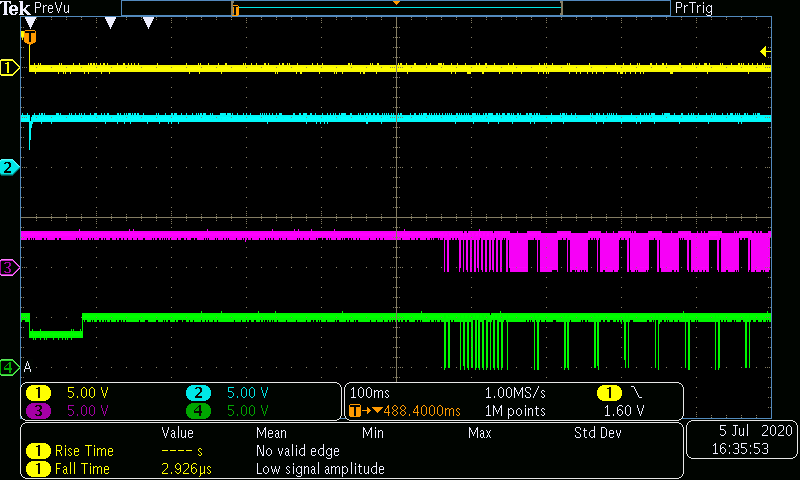
\includegraphics[width = \textwidth]{graphics/ATMega2560_DTR_RESET_RX_TX_gesamt}
\caption{Hochladen des Programmcodes auf den ATMega2560.}
\label{fig:ATMega2560_DTR_RESET_RX_TX_gesamt}
\end{figure}

\begin{figure}[h!]
\center
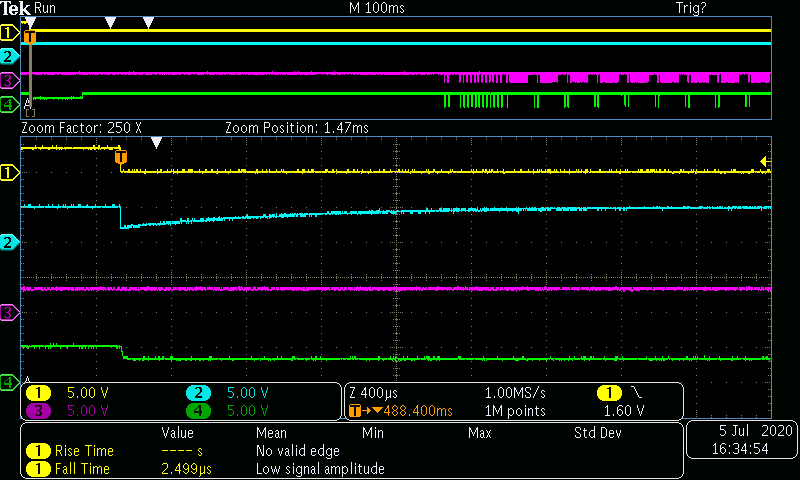
\includegraphics[width =  \textwidth]{graphics/ATMega2560_DTR_RESET_RX_TX_1}
\caption{Handshake zum Hochladen des Programmcodes auf den ATMega2560. Zoom auf den Moment des Resets.}
\label{fig:ATMega2560_DTR_RESET_RX_TX_1}
\end{figure}
\newpage
\item ESP32\\

Um herauszufinden, ob und wie der Handshake durchgeführt wird, wurde beim Hochladen eines Programms an den folgenden Leitungen gemessen:\\

\begin{tabular}{lcl}
1 & Gelb & RTS\\
2 & Blau & DTR\\
3 & Violett & EN\\
4 & Grün & IO0\\
\\
\end{tabular}

In Abbildung \ref{fig:ESP32_RTS_DTR_EN_IO0_gesamt} wurden die ersten 100ms des Hochladen eines Programms auf das ESP32 gemessen. Gesucht wird nach einem gleichzeitigen Flankenwechsel der RTS-Leitung von 0 auf 1 und der DTR-Leitung von 1 nach 0. Abbildung \ref{fig:ESP32_RTS_DTR_EN_IO0_2} zeigt eine genauere Aufnahme zum Zeitpunkt des Flankenwechsels.

Was auffält, ist dass entgegen der Erwartung der Flankenwechsel der beiden Leitungen leicht verzögert ist (um ca. 80 \textmu s). Auch das Signal des EN-Pins erreicht wesentlich schneller einen HIGH-Zustand als erwartet. Denn gemäss der Theorie müssen die Pins EN und IO0 zum gleichen Zeitpunkt auf LOW sein, um in den Download-Boot-Modus zu kommen, und trotz der Abweichung der Praxis zur Theorie funktioniert die Übertragung des Codes. Ein Fehler in der Matrix?

\newpage
\begin{table}[h!]
\center
\begin{tabular}{lcl|lcl|lcl|lcl}
1 & Gelb & RTS & 2 & Blau & DTR & 3 & Violett & EN & 4 & Grün & IO0\\
\end{tabular}
\end{table}
\begin{figure}[h!]
\center
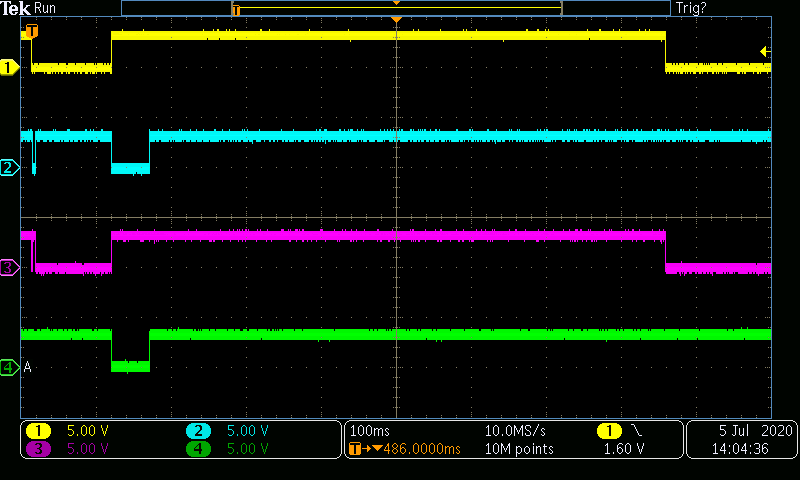
\includegraphics[width = \textwidth]{graphics/ESP32_RTS_DTR_EN_IO0_gesamt}
\caption{Handshake zum Hochladen des Programmcodes auf das ESP32.}
\label{fig:ESP32_RTS_DTR_EN_IO0_gesamt}
\end{figure}

\begin{figure}[h!]
\center
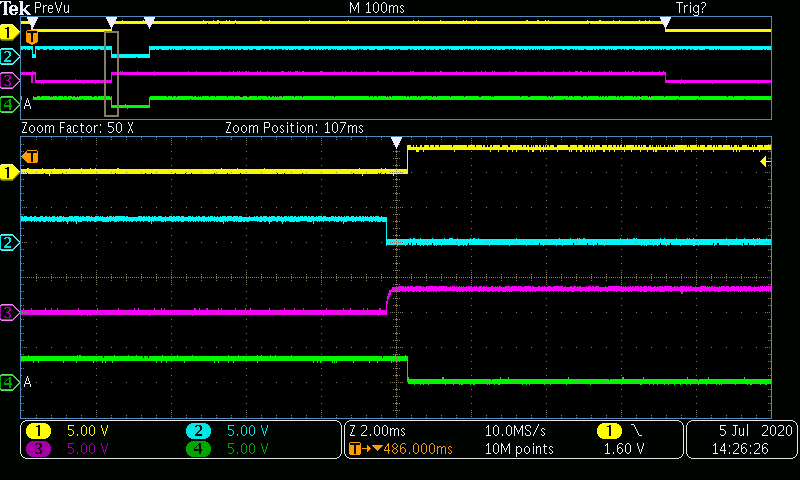
\includegraphics[width = \textwidth]{graphics/ESP32_RTS_DTR_EN_IO0_2}
\caption{Handshake zum Hochladen des Programmcodes auf das ESP32. Zoom auf gleichzeitiger Flankenwechsel RTS und DTR.}
\label{fig:ESP32_RTS_DTR_EN_IO0_2}
\end{figure}

\newpage

In einem Forum\footnote{https://forum.micropython.org/viewtopic.php?t=4607} wurde diese Auffälligkeit auch schon besprochen. Die Diskussion führte zum selben Ergebnis wie bei Inbetriebnahme. Nämlich, dass es nach dem Reset eine Zeit dauert, bis im Startprozess die Pins geprüft werden. Dazu gehört auch der Pin IO0. Somit ist es möglich, den Pin IO0 kurz nach dem Reset auf 0 zu ziehen.
Im selben Forum wurde auch die in Abbildung \ref{fig:ESP32_Handshake_Forum} gezeigte Darstellung gefunden. Ein Kommentar weist darauf hin, das mit dem esptool.py der EN-Pin des ESP32 direkt auf RTS gehängt werden kann. So lassen sich die Zeitpunkte, zu der die Pins auf 0 sind, näher zusammenschieben.

\begin{figure}[h!]
\center
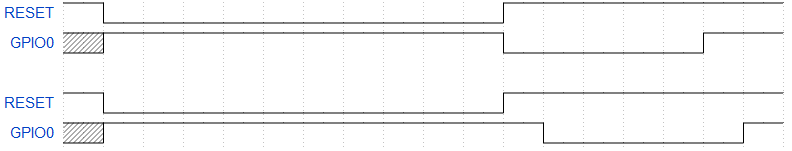
\includegraphics[width = \textwidth]{graphics/ESP32_Handshake_Forum}
\caption{Handshake zum Hochladen des Programmcodes auf das ESP32. Zoom auf gleichzeitiger Flankenwechsel RTS und DTR.}
\label{fig:ESP32_Handshake_Forum}
\end{figure}

Die Messung nach dem Einlöten der Brücke bestätigt dies, wie in Abbildung \ref{fig:ESP32_RTS_DTR_EN_IO0_mit_Bruecke_1} ersichtlich ist. Allerdings spielt der Kondensator jetzt nicht mehr so eine grosse Rolle, was auch nicht nötig ist. Auf das Hochladen des Codes hat die Brücke keinen Einfluss. Die Funktioniert wie bei der Schaltung ohne Brücke einwandfrei.
\begin{table}[h!]
\center
\begin{tabular}{lcl|lcl|lcl|lcl}
1 & Gelb & RTS & 2 & Blau & DTR & 3 & Violett & EN & 4 & Grün & IO0\\
\end{tabular}
\end{table}
\begin{figure}[h!]
\center
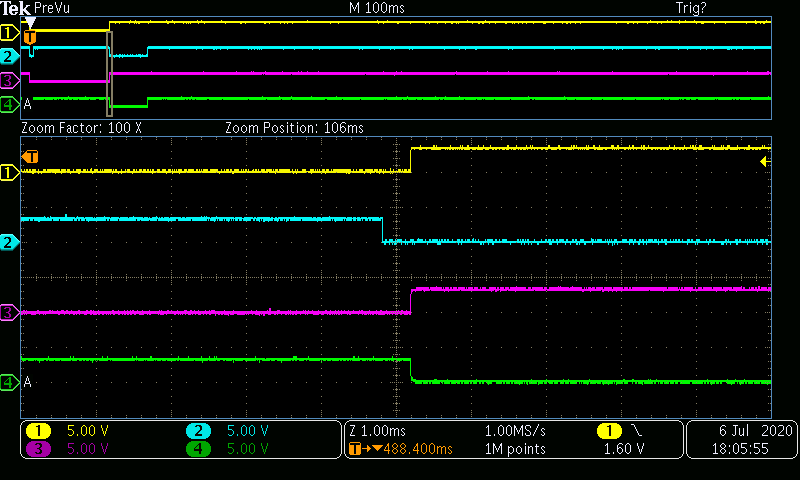
\includegraphics[width = \textwidth]{graphics/ESP32_RTS_DTR_EN_IO0_mit_Bruecke_1}
\caption{Handshake zum Hochladen des Programmcodes auf das ESP32. Zoom auf gleichzeitiger Flankenwechsel RTS und DTR.}
\label{fig:ESP32_RTS_DTR_EN_IO0_mit_Bruecke_1}
\end{figure}
\end{enumerate}

\end{enumerate}
